\chapter{The macOS port}
\label{ch:macport}

The folder \file{mac} of the repository contains a second implementation of Texture Explorer,
for macOS and Apple's graphics interface, Metal. It is the same program: the same panels and
controls, the same defaults, the same materials (the folder \file{assets} is shared) and, above
all, the same formulas. Figure~\ref{fig:macpyramid} shows it in the situation of
Figure~\ref{fig:pyramid}.

\begin{figure}[ht]
  \centering
  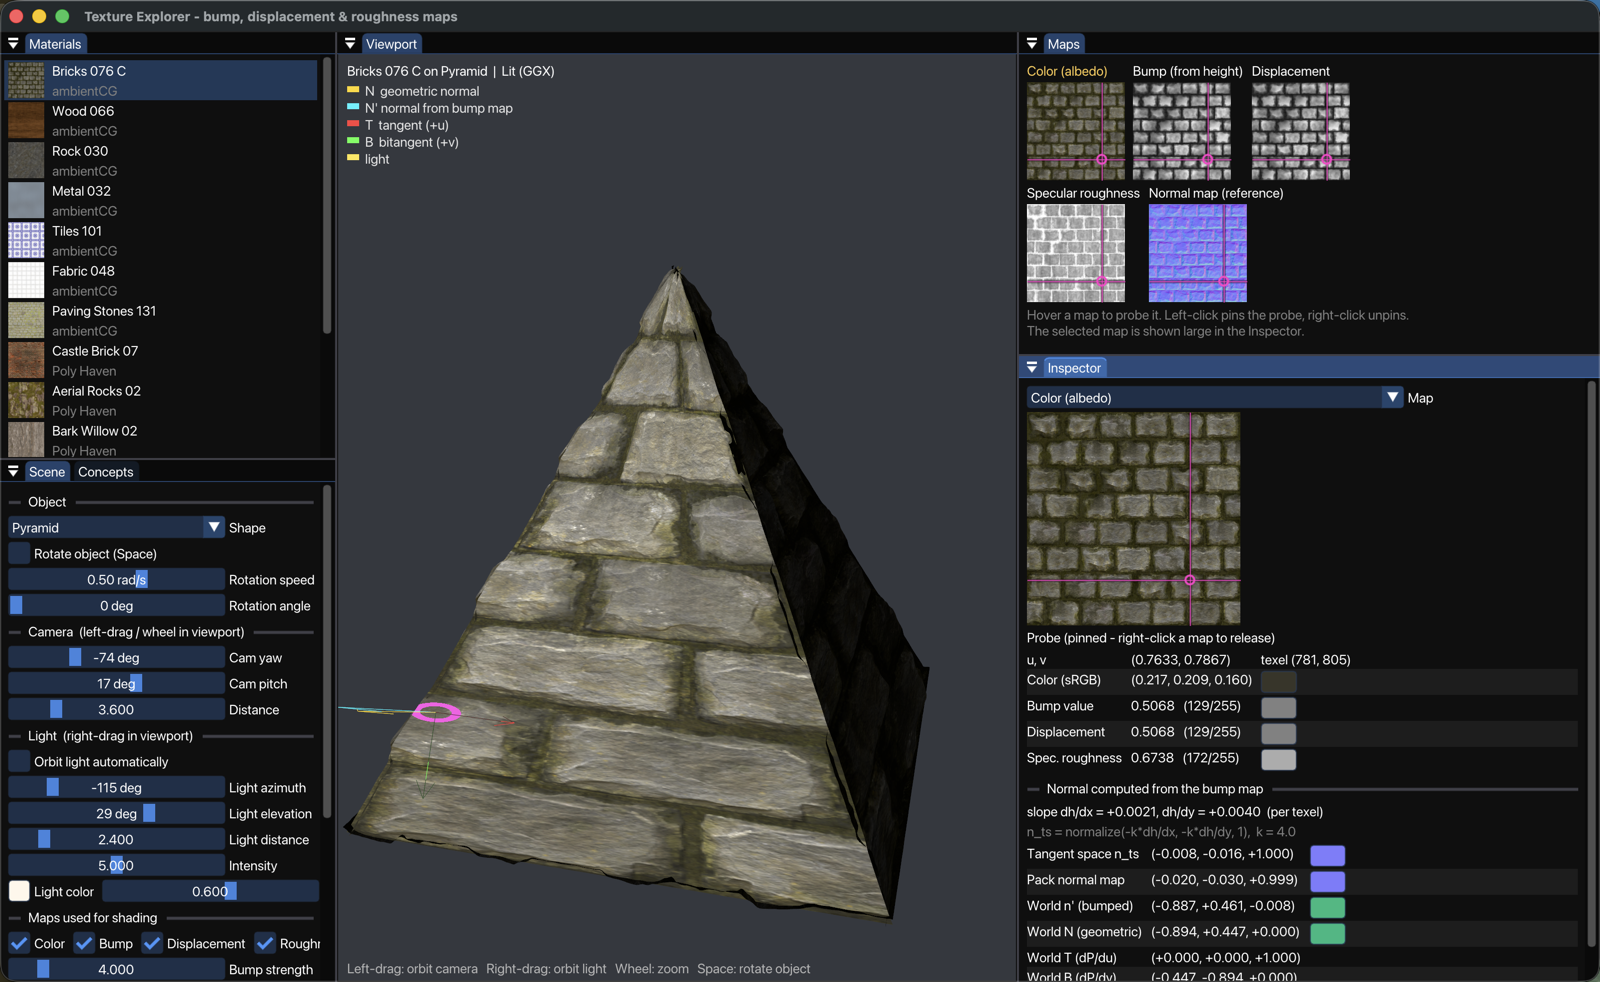
\includegraphics[width=\linewidth]{figures/pyramid-probe-mac.png}
  \caption{The macOS version in the situation of Figure~\ref{fig:pyramid}: same material,
  shape, camera and light, with the probe pinned near the same texel. The geometric normal
  $\Nv=(-0.894, 0.447, 0.000)$ is the same in both inspectors.}
  \label{fig:macpyramid}
\end{figure}

The port was written so that it can be read next to the original: every file of \file{src}
has a counterpart with the same name in \file{mac/src}, with the same classes and functions in
the same order. Only four layers of the program depend on the platform, and each is replaced
by its macOS counterpart (Table~\ref{tab:layers}). This chapter goes through them; the next
one explains how to compare the two implementations.

\begin{table}[ht]
\centering\small
\begin{tabularx}{\linewidth}{@{}lllX@{}}
\toprule
\textbf{Layer} & \textbf{Windows} & \textbf{macOS} & \textbf{Where}\\
\midrule
vectors and matrices & DirectXMath & \code{simd} & \file{mac/src/VecMath.h}, everywhere\\
GPU interface & Direct3D~11 & Metal (metal-cpp) & \file{Renderer.*}, \file{Material.cpp}\\
shading language & HLSL & Metal Shading Language & \file{mac/shaders/*.metal}\\
window and events & Win32 & AppKit, MetalKit & \file{main.mm}\\
\bottomrule
\end{tabularx}
\caption{The four platform layers of Texture Explorer. Dear ImGui, \code{stb\_image} and
\code{nlohmann/json} are used unchanged; ImGui has back ends for both systems.}
\label{tab:layers}
\end{table}

Metal is an Objective-C interface, but Apple publishes \emph{metal-cpp}, a header-only C++
wrapper in which every Metal object is a C++ class: \code{MTL::Device}, \code{MTL::Texture},
\code{MTL::RenderCommandEncoder}, and so on. With it, the whole port except \file{main.mm} is
plain C++20, and the Direct3D and Metal versions of a function can be compared line by line.

\section{Building and running}
The port needs macOS~13 or later, Xcode or its command-line tools, and CMake. The materials are
already in the repository. From its root:
\begin{lstlisting}[language={},numbers=none,frame=none,basicstyle=\ttfamily\small]
cmake -S mac -B mac/build -DCMAKE_BUILD_TYPE=Release
cmake --build mac/build
open mac/build/TextureExplorer.app
\end{lstlisting}
The controls are those of Chapter~\ref{ch:intro}; on a Mac the shaders are reloaded with F5
(fn-F5 on most keyboards) or Command-R. The program finds \file{assets} and
\file{mac/shaders} by walking up from the application bundle, so the shaders can be edited in
place while it runs.

\section{Vectors and matrices}
\label{sec:simd}
DirectXMath does not exist on macOS. Its replacement is Apple's \code{simd} library, whose types
\code{simd::float3}, \code{simd::float4x4}, \dots{} have the same names as the vector types of
the Metal Shading Language. Two differences matter.

\paragraph{Storage.} DirectXMath distinguishes a computing type, \code{XMVECTOR} (a SIMD
register), from storage types such as \code{XMFLOAT3} (three packed floats), and converts with
\code{XMLoadFloat3} and \code{XMStoreFloat3}. A \code{simd::float3} is both, but it occupies 16
bytes, so a vertex built from it would not have the packed 48-byte layout of the Direct3D
version. The port therefore computes with \code{simd::float3} and stores GPU data in two small
structures, \code{Float3} and \code{Float4}, which convert to and from \code{simd} implicitly.
The code becomes shorter: compare the sides of the pyramid in the two versions, where
\code{XMLoadFloat3}, \code{XMVectorLerp} and \code{XMStoreFloat3} simply disappear.

\paragraph{Row and column vectors.} DirectXMath multiplies a \emph{row} vector by a matrix,
$\vect p'=\vect pM$; \code{simd}, like Metal and most mathematics texts, multiplies a matrix by
a \emph{column} vector, $\vect p'=M\vect p$. Each matrix of one convention is the transpose of
the corresponding matrix of the other, and products are written in the opposite order:
\[
  \vect p_{\mathrm{clip}} = \vect p\,(W\,V\,P) \quad\text{(Windows)},\qquad
  \vect p_{\mathrm{clip}} = (P\,V\,W)\,\vect p \quad\text{(macOS)}.
\]
\file{mac/src/VecMath.h} defines the few constructors the program needs, each the transpose of
its DirectXMath namesake. For example, the view matrix has the camera's axes as its rows:

\excerpt{mlookat}

The projection matrix carries over unchanged because Metal shares two conventions with Direct3D:
clip-space depth runs from $0$ at the near plane to $1$ at the far plane (OpenGL uses $-1$ to
$1$), and the origin of a texture is its top-left corner, with $v$ growing downwards
(Section~\ref{sec:uvconv}). Everything that Part~I says about texture space therefore holds on
both systems, and the patch functions of Chapter~\ref{ch:geometry} are the same; only their
vector types change.

\excerpt{mperspective}

\section{From HLSL to the Metal Shading Language}
\label{sec:msl}
The Metal Shading Language (MSL) is a dialect of C++14 with vector types named like HLSL's,
so the translation of \file{shaders/pbr.hlsl} into \file{mac/shaders/pbr.metal} is close to
mechanical. Table~\ref{tab:hlslmsl} lists every kind of change it needed. The mathematics---the
displacement, the central differences, the TBN matrix, the GGX/Cook--Torrance BRDF---is
identical, statement by statement.

\begin{table}[ht]
\centering\small
\begin{tabularx}{\linewidth}{@{}>{\raggedright\arraybackslash}X>{\raggedright\arraybackslash}X@{}}
\toprule
\textbf{HLSL} (\file{shaders/pbr.hlsl}) & \textbf{MSL} (\file{mac/shaders/pbr.metal})\\
\midrule
\code{cbuffer Frame : register(b0) \{...\}} & \code{struct Frame \{...\}}, passed as \code{constant Frame\& f [[buffer(1)]]}\\
\code{Texture2D colorMap : register(t0);} (global) & \code{texture2d<float> colorMap [[texture(0)]]} (function parameter)\\
\code{SamplerState linearWrap : register(s0);} & \code{sampler linearWrap [[sampler(0)]]}\\
semantics \code{POSITION}, \code{NORMAL}, \dots & \code{[[attribute(0)]]}, \code{[[attribute(1)]]}, \dots{} with \code{[[stage\_in]]}\\
\code{SV\_Position}, \code{SV\_Target} & \code{[[position]]}; the return value of a \code{fragment} function\\
entry point chosen by the compiler call & keywords \code{vertex} and \code{fragment}\\
\code{mul(v, M)} with \code{row\_major} & \code{M * v}\\
\code{lerp}, \code{frac} & \code{mix}, \code{fract}\\
\code{t.SampleLevel(s, uv, l)} & \code{t.sample(s, uv, level(l))}\\
\code{t.GetDimensions(w, h)} & \code{t.get\_width()}, \code{t.get\_height()}\\
\code{r.xxx} (swizzle of a scalar) & \code{float3(r)}\\
\code{float3} in a constant buffer (12 bytes) & \code{packed\_float3} (a \code{float3} takes 16 bytes)\\
\bottomrule
\end{tabularx}
\caption{The changes made in translating the shaders from HLSL to MSL.}
\label{tab:hlslmsl}
\end{table}

\paragraph{Resources are parameters.} The most visible change is that textures, samplers and
constants are not global variables bound to registers but parameters of the shader functions,
with the binding number as an attribute. A helper function such as \code{BumpNormalTS} cannot see
the resources of its caller, so they are passed to it explicitly:

\excerpt{mbumpnormalts}

\paragraph{The layout of the constants.} An HLSL constant buffer packs a \code{float3} into 12
bytes and lets the next \code{float} complete the 16-byte row. In MSL, as in C++ with
\code{simd}, a \code{float3} is aligned to 16 bytes; MSL's \code{packed\_float3} restores the
HLSL behaviour. With it, the structure has the rows of the \code{cbuffer} of
Chapter~\ref{ch:shaders}, 240 bytes in both versions, and the C++ structure uses \code{Float3} in
the same places. Its \code{static\_assert} now checks the size and one offset exactly:

\excerpt{mframe}

\excerpt{mframeconstants}

The vertex shader shows the remaining differences: semantics replaced by attributes, the
constants reached through \code{f}, and products in the column order.

\excerpt{mvsmain}

\section{Textures}
\label{sec:mactextures}
Direct3D separates a texture (memory) from its \emph{views} (interpretations of that memory);
Section~\ref{sec:typeless} used a typeless texture with a \code{UNORM} view for the interface and
a \code{UNORM\_SRGB} view for shading. Metal has only textures, but a texture created with the
usage flag \code{PixelFormatView} can produce another texture that is a view of the same memory
with a different pixel format. The colour map is therefore an \code{RGBA8Unorm} texture plus an
\code{RGBA8Unorm\_sRGB} view of it, which decodes sRGB when sampled, exactly as in Direct3D.
The CPU copy for the inspector is unchanged.

\excerpt{mloadimage}

Two other differences appear here. The pixels are written with \code{replaceRegion} into a
\emph{managed} texture, one that has a copy the CPU can write (on a Mac with Apple silicon the
CPU and the GPU share the memory, and the copy costs nothing). And the mipmaps are generated by
a command recorded into a \emph{command buffer}, which brings us to the main difference between
the two interfaces.

\section{The renderer}
\label{sec:macrenderer}
Table~\ref{tab:d3dmetal} is a dictionary of the concepts the renderer uses. The deepest
difference is in its second row. A Direct3D~11 \emph{immediate context} executes every call as
it is made, as far as the program can tell. Metal makes the recording of GPU work explicit: the
program takes a \emph{command buffer} from a \emph{command queue}, records passes into it through
\emph{encoders}, and \emph{commits} it; the GPU executes committed buffers in order. In Texture
Explorer each frame has one command buffer, which receives first the render pass of the scene
and then the render pass of the interface.

\begin{table}[ht]
\centering\small
\begin{tabularx}{\linewidth}{@{}>{\raggedright\arraybackslash}X>{\raggedright\arraybackslash}X@{}}
\toprule
\textbf{Direct3D 11} (\file{src/Renderer.cpp}) & \textbf{Metal} (\file{mac/src/Renderer.cpp})\\
\midrule
\code{ID3D11Device} & \code{MTL::Device}\\
immediate context (\code{ID3D11DeviceContext}) & command queue, command buffers, encoders\\
swap chain, \code{Present} & drawables of the \code{MTKView}, \code{presentDrawable}\\
texture + shader resource view & texture, possibly a view of another texture\\
render target and depth-stencil views & attachments of a render pass descriptor\\
\code{ClearRenderTargetView} & load action \code{Clear}\\
\code{ResolveSubresource} & store action \code{MultisampleResolve}\\
shaders + input layout + blend state & one render pipeline state\\
input layout (\code{D3D11\_INPUT\_ELEMENT\_DESC}) & vertex descriptor (attributes by number)\\
rasterizer state & \code{setCullMode}, \code{setViewport} on the encoder\\
depth-stencil state, sampler state & the same, created from descriptors\\
dynamic constant buffer, \code{Map(WRITE\_DISCARD)} & \code{setVertexBytes}, \code{setFragmentBytes}\\
dynamic vertex buffer & a new buffer per frame\\
\code{D3DCompileFromFile} & \code{newLibrary} from source text\\
\code{ComPtr} & \code{NS::SharedPtr}\\
\bottomrule
\end{tabularx}
\caption{Direct3D~11 and Metal concepts used by the renderer.}
\label{tab:d3dmetal}
\end{table}

\paragraph{Pipeline states.} Direct3D~11 lets the program combine shaders, input layout, blend
state and target formats freely at draw time. Metal, like Direct3D~12 and Vulkan, requires the
combination to be declared in advance and compiled once into an immutable \emph{render pipeline
state}, which therefore also names the formats of the targets: four samples per pixel, an sRGB
colour target and a 32-bit depth buffer. The lines get a second pipeline state, which is the
first one with blending enabled.

\excerpt{mpipeline}

\paragraph{The off-screen target} has the same three parts as in Direct3D: a multisampled
colour texture, a multisampled depth texture and a resolved single-sample texture, with a
non-sRGB view of the latter for the interface.

\excerpt{mscenetarget}

\paragraph{Drawing.} A render pass states what happens to each attachment at its start
(\emph{load action}) and end (\emph{store action}). Clearing is a load action, and the resolve of
the multisampled image is a store action, so there is no \code{ClearRenderTargetView} and no
\code{ResolveSubresource}. The depth buffer is not needed after the pass and is not stored at
all, which saves memory traffic, particularly on Apple GPUs, which keep the attachments of a
pass in on-chip memory. The constants are copied into the command buffer with
\code{setVertexBytes} rather than written into a buffer, because Metal does not rename memory
behind the program's back as \code{Map(WRITE\_DISCARD)} does; for the same reason the lines go
into a new small buffer each frame. Nothing needs to be unbound at the end: Metal tracks by
itself which passes write and which read each resource.

\excerpt{mrenderscene}

\section{The window and the frame}
\label{sec:macframe}
The Windows program owns its main loop: it processes the window's messages and then draws a
frame, over and over. A Mac program is organized the other way round. The application object
of AppKit owns the loop, and the program supplies a \emph{delegate} whose methods are called
when something happens. Drawing is driven the same way: a \code{MTKView} owns the drawable
images of the window (the counterpart of the swap chain) and calls its delegate once per refresh
of the display. That method, in \file{main.mm}, replaces the body of the Windows loop:

\excerpt{mframeloop}

Asking the view for its render pass descriptor may wait until the display releases a drawable;
this ties the frame rate to the display, as \code{Present(vsync)} does on Windows. The
\code{@autoreleasepool} releases at the end of the frame every object that Metal and AppKit
returned without handing it to the program (the command buffer, the encoders, the
descriptors). \file{main.mm} is the only file in Objective-C++; the casts written
\code{(\_\_bridge T)p} convert between metal-cpp pointers and Objective-C references, which
designate the same objects.

\paragraph{Points and pixels.} One change in the interface has nothing to do with Metal. On
macOS, Dear ImGui measures the screen in \emph{points}, and a Retina display has two pixels per
point in each direction. The scene is therefore rendered at the size of the Viewport panel in
pixels---\code{DisplayFramebufferScale} times its size in points---and shown at its size in
points, so that it is as sharp as the Windows image. On Windows the factor is~1.

\excerpt{mviewportsize}
